\section{Discrete-time Markov chains}
We begin by introducing discrete Markov chain concepts that will be used to study the properties of temporally regularized MDPs. In this thesis, we focus on discrete Markov chains, however the concepts can be extended to the continuous case.\\ Discrete Markov chain are stochastic models representing sequences of random variable satisfying the Markov property. Formally, we define a discrete-time Markov chain (\cite{norris1998markov,levin2017markov,bremaud2013markov})  with finite state space $\s$ by a sequence of $|\s|-$valued random variable $X_0,X_1,..$. and a transition function $\p : \s \times \s \mapsto [0,1]$. The sequence of random variable needs to satisfy the Markov property:
\begin{definition}
A stochastic process satisfy Markov property if:
\begin{equation}
    \p (X_{n+1}=j|X_n = i,X_{n-1}=k,...) = \p (X_{n+1}=j|X_n = i)
\end{equation}
\end{definition}
Intuitively, this means that the probability of moving to the next states is based solely on its present state and not its history. One of the most studied Markov chains considers the property of randomly walking on a chain as described in figure (\ref{fig:random_walk}).\\
\begin{figure}
    \centering
    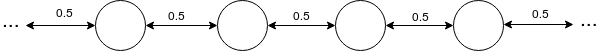
\includegraphics[scale=0.7]{fig/Markov_chain.png}
    \caption{Random walk}
    \label{fig:random_walk}
\end{figure}
Discrete time Markov chains can also be represented in matrix form. The transition function can be represented as a $|\s| \times |\s|$ matrix P such that $P_{ij} = \p(X_{n+1}=j|X_n=i)$. Studying Markov chains from an algebraic perspective can sometimes simplify the analysis.  \\
We now define some useful fundamental properties of Markov chains.
If every state is accessible from every other, the chain(or its transition matrix) is said to be irreducible. 
\begin{definition}
A chain is said to be irreducible if $\forall i,j \in \s$ there exists $n \in \mathbb{N}$ such that:
\begin{equation}
      \quad P(X_n = j|X_0=i) > 0
\end{equation}
\end{definition}
\begin{definition}
The period of a state is the greatest common divisor of the set {$n \in  \mathbb{N} : \quad P(X_n=i|X_0=i) > 0$}. The chain is defined as aperiodic if every state has period 1.
\end{definition}
\begin{definition}
Let $T_i$ define the hitting time of state i such that:
\begin{equation}
    T_i = inf(n \geq 1 : X_n = i | X_0 = i)
\end{equation}
We define a transient state if $T_i$ is not finite. A state is called recurrent if it is not transient.
\end{definition}
\begin{definition}
A chain is defined as ergodic if it is positive recurrent and aperiodic.
\end{definition}
Throughout this thesis, we make the following mild assumption on the Markov chain:
\begin{assumption}
P is ergodic
\end{assumption}
Most of the Reinforcement learning theory relies on this assumption. However, some works considers the case when the chain is not ergodic (\cite{leike2016nonparametric}).

\section{Stationary distribution}
It is often interesting to study the properties of Markov chains in the limit. We define the stationary distribution $\mu_i$ as the \emph{proportion of time} spend in each state $i \in \s$.
\begin{definition}
Assuming that P is ergodic, P has a unique stationary distribution $\mu$ that satisfies:
\begin{equation}
\begin{split}
    \mu &= \mu P \\
    \sum_i \mu_i &= 1
\end{split}
\end{equation}
\end{definition}
There exists many different metrics used to define distance's from stationary distribution (\cite{levin2017markov}). One common metric in discrete Markov chains can be defined as follows:
\begin{equation}
    d_t(P) = \norm{P^t \mathbbm{1} - \mu}_{ \infty } 
    \label{eq:d_markov}
\end{equation}
where $\mathbbm{1}$ is a vector of one's.
\section{Detailed Balance}
The concept of detailed balance originated from physics. It is used to study the behavior of systems in the limit at \emph{equilibrium}. 
\begin{definition}[Detailed balance~\cite{kemeny1976finite}]
Let $P$ be an irreducible Markov chain with invariant stationary distribution $\mu$. $\mu_i$ defines the $i$th element of $\mu$. A chain is said to satisfy detailed balance if and only if
\begin{equation}
    \mu_i P_{ij} = \mu_j P_{ji} \qquad \forall i,j \in \s.
\end{equation}
\end{definition}
Intuitively, this means that if we start the chain in a stationary distribution, the amount of probability that flows from $i$ to $j$ is equal to the one from $j$ to $i$. In other words, the system must be at equilibrium. An intuitive example of a physical system not satisfying detailed balance is a snow flake in a coffee. 
\begin{remark}
If a chain satisfies detailed balance, it is called reversible.
\end{remark}

\section{Mixing Time}

In Markov chains theory, one of the main challenges is to study the mixing time of the chain (\cite{levin2017markov}). The mixing time corresponds to the time needed for the chain to be \emph{close} to its stationary distribution $\mu$. More formally it can be defined as:
\begin{equation}
    t_{mix}(\epsilon) = \text{min} \{ t : d_t(P) < \epsilon \}
\end{equation}
where $d_t(P)$ can be defined as in (\ref{eq:d_markov}).\\
When the chain is reversible, it is possible to estimate and bound the mixing time relatively efficiently (\cite{diaconis1991geometric,}). Indeed, many chains do not satisfy this detailed balance property. In this one case it is possible to use a different, but related, chain called the reversal Markov chain to infer mixing time bounds (\cite{fill1991eigenvalue,chung2012chernoff}).




\section{Reversal Markov Chains}
The reversal Markov chain $\widetilde{P}$ can be interpreted as the Markov chain $P$ with time running backwards. It is be a key concept used to define convergence and bias induced by temporal regularization later in this thesis. 
\begin{definition}[Reversal Markov chain~\cite{kemeny1976finite}]
Let $\widetilde{P}$ the reversal Markov chain of $P$ be defined as:
\begin{equation}
    \widetilde{P_{ij}} = \frac{\mu_j P_{ji}}{\mu_i} \qquad \forall i,j \in \s.
\end{equation}
\end{definition}
As an example, assuming a Markov chain P has a uniform stationary distribution, if a transition is highly irreversible like falling off a cliff ($P_{ij} \# P_{ji}$) the difference between the forward and the backward chain in that state will be high. We now introduce some properties of reversal Markov chains that will be used later in the thesis.
\begin{remark}
If $P$ is irreducible with invariant distribution $\mu$, then $\widetilde{P}$ is also irreducible with invariant distribution $\mu$.
\end{remark}

\begin{remark}
If $P$ is reversible than $P = \widetilde{P}$
\end{remark}
Furthermore, both $P$ and $\widetilde{P}$ have the same stationary distribution and so does any convex combination of them.

\begin{lemma}
$P$ and $(1-\param) P + \param \widetilde{P}$ have the same stationary distribution $\mu \quad \forall \param \in [0,1]$.
\end{lemma}
\begin{proof}
\begin{equation}
    \begin{split}
        \mu ( (1-\param) P + \param \widetilde{P}) &=  (1-\param) \mu P + \param \mu \widetilde{P} \\
        &= (1-\param)\mu + \param \mu\\
        &= \mu.
    \end{split}
\end{equation}
\end{proof}


